%%==============================================================
%% Modelo de TCC para o curso de Sistemas de Informação
%% da Universidade Federal de Viçosa - Campus de Rio Paranaíba
%% Autor: Rodrigo Smarzaro (smarzaro@ufv.br)
%% Última versão Setembro/2019
%% Arquivo em formato UTF-8
%% Compilar com pdftex e biber
%% Precisa do arquivo abntex2-UFV.sty
%%==============================================================

\documentclass[
    % -- opções da classe memoir --
    12pt,                   % tamanho da fonte
    openright,              % capítulos começam em página ímpar (insere página vazia caso preciso)
    oneside,                % para impressão só no anverso. Oposto a twoside
    a4paper,                % tamanho do papel.
    % -- opções do pacote abntex2 --
    % chapter=TITLE,        % Títulos em maiúsculas
    sumario=tradicional,    % Sumário padrão memoir 
    % -- opções do pacote babel --
    english,                % idioma adicional para hifenização
    brazil,                 % idioma principal do documento
    ]{abntex2}

% Pacotes fundamentais
\usepackage{abntex2-UFV}        % Personalização para a Universidade Federal de Viçosa
\usepackage{lmodern}            % Usa a fonte Latin Modern
\usepackage[T1]{fontenc}        % Seleção de códigos de fonte de saída
\usepackage[utf8]{inputenc}        % Codificação do documento (conversão automática dos acentos)
\usepackage{indentfirst}        % Indenta o primeiro parágrafo de cada seção.
\usepackage{graphicx}            % Inclusão de gráficos
\usepackage{booktabs}           % \toprule, \midrule e \bottomrule para tabelas
\usepackage{csquotes}

% Sistema autor-data com títulos nas referências em negrito
%\usepackage{url}

% ---
\usepackage[brazilian,hyperpageref]{backref}    % Paginas com as citações na bibl
% Configurações do pacote backref
% Usado sem a opção hyperpageref de backref
\renewcommand{\backrefpagesname}{Citado na(s) página(s):~}
% Texto padrão antes do número das páginas
\renewcommand{\backref}{}
% Define os textos da citação
\renewcommand*{\backrefalt}[4]{
   \ifcase #1 %
       Nenhuma citação no texto.%
   \or
       Citado na página #2.%
   \else
       Citado #3 vezes nas páginas #2.%
   \fi}%
% ---


\usepackage[alf,abnt-emphasize=bf]{abntex2cite}
%\usepackage[backend=biber,style=abnt,uniquename=init,giveninits,repeatfields]{biblatex}
%\\addbibresource{referencias.bib}
%\\usepackage{url}
%\\makeatletter
%\\g@addto@macro{\UrlBreaks}{\UrlOrds}
%\\makeatother

%\setlength\bibparsep{10pt}

% ---
% CONFIGURAÇÕES DE PACOTES
% ---

% Informações de dados para CAPA e FOLHA DE ROSTO
\titulo{Computação Afetiva: Panorama das principais pesquisas publicadas no Brasil e Discussão Ética}
\autor{Ana Flávia Morais Santos - 187\\Gleidson Vinícius Gomes Barbosa – 6331}
\local{Rio Paranaíba}
\data{2019}
\orientador{Nome do Orientador}    % redefinido no abntex2-UFV para aceitar Instituição (default = UFV-CRP)
%\coorientador{Nome do Coorientador}
\instituicao{Universidade Federal de Viçosa}

\campus{\emph{Campus} de Rio Paranaíba}      % pacote abntex2-UFV
\curso{Sistemas de Informação}               % pacote abntex2-UFV
\membrobancaA{Membro da Banca A}             % pacote abntex2-UFV default = UFV-CRP
\membrobancaB[UFMG]{Membro da Banca B}       % pacote abntex2-UFV default = UFV-CRP
\databanca{\today}                           % pacote abntex2-UFV

% O preambulo deve conter o tipo do trabalho, o objetivo,
% o nome da instituição e a área de concentração
\preambulo{Monografia apresentada à Universidade Federal de Viçosa, como parte das exigências para a a aprovação na disciplina Trabalho de Conclusão de Curso I}
% ---

% ---
% Configurações de aparência do PDF final

% informações para o arquivo pdf de saída
% Interessante alterar a cor dos links para preto(black)
% na versão final para imprimir
\makeatletter
\hypersetup{
        % metadados
        pdftitle={\@title},
        pdfauthor={\@author},
        pdfsubject={\imprimirpreambulo},
        pdfcreator={LaTeX with abnTeX2},
        colorlinks=true,   % false: links em frame; true: links coloridos
        linkcolor=black,   % cor dos links no documento
        citecolor=blue,    % cor dos links para a bibliografia
        filecolor=magenta, % cor dos links para arquivos
        urlcolor=blue,     % cor dos links para sites
        bookmarksdepth=4   % profundidade do sumário do PDF
}
\makeatother
% ---

\begin{document}
% Retira espaço extra obsoleto entre as frases.
\frenchspacing

% ----------------------------------------------------------
% ELEMENTOS PRÉ-TEXTUAIS
% ----------------------------------------------------------
\pretextual

% Capa
\imprimircapa

% Folha de rosto
\imprimirfolhaderosto
% ---

% Inserir folha de aprovação
\imprimirfolhadeaprovacao

% Dedicatória
\begin{dedicatoria}
   \vspace*{\fill}
   \centering
   \noindent
   \textit{Texto qualquer da dedicatória}
   \vspace*{\fill}
\end{dedicatoria}
% ---

% Agradecimentos
\begin{agradecimentos}
%Insira o texto de agradecimentos aqui
\end{agradecimentos}
% ---

% Epígrafe
\begin{epigrafe}
    \vspace*{\fill}
    \begin{flushright}
        \textit{``Word? nunca mais.''\\
        (Qualquer usuário de \LaTeX)}
    \end{flushright}
\end{epigrafe}
% ---

% RESUMOS

% resumo em português
\begin{resumo}
 \noindent
%Insira o resumo aqui

 \vspace{\onelineskip}

 \noindent
 \textbf{Palavras-chaves}: computação afetiva, ética, IHC, educação.
\end{resumo}

% resumo em inglês
\begin{resumo}[Abstract]
\begin{otherlanguage*}{english}
   \noindent
%Insira o abstract aqui

   \vspace{\onelineskip}

   \noindent
   \textbf{Key-words}: affective computing, ethic, HCI, education.
 \end{otherlanguage*}
\end{resumo}

% inserir lista de ilustrações
\pdfbookmark[0]{\listfigurename}{lof}
\listoffigures*
\cleardoublepage
% ---

% inserir lista de tabelas
\pdfbookmark[0]{\listtablename}{lot}
\listoftables*
\cleardoublepage
% ---

% Lista de siglas e abreviaturas (opcional)
% sintaxe: \item [sigla] Descrição da sigla

%\begin{siglas}
%\item[ABNT] Absurdas Normas Técnicas
%\item[UFV] Universidade Federal de Viçosa
%\item[CRP] \emph{Campus} de Rio Paranaíba
%\end{siglas}

% Lista de símbolos (opcional)
% sintaxe: \item [simbolo] Descrição do símbolo

%\begin{simbolos}
%\item[$\infty$ ] Infinito
%\end{simbolos}

% inserir o sumario
\pdfbookmark[0]{\contentsname}{toc}
\tableofcontents*
\cleardoublepage
% ---

% ----------------------------------------------------------
% ELEMENTOS TEXTUAIS
% ----------------------------------------------------------
\textual

%Modifique a estrutura dos capítulos e seções de acordo com a necessidade do seu trabalho
\chapter{Introdução}\label{sec:introducao}
A realidade em que vivemos é marcada pela internet e são muitas as formas de interação entre os seres humanos e as máquinas. Da percepção de tais acontecimentos,  \citeonline{squirra2016tecnologia} apresenta os sentidos humanos caminhando rumo a uma inédita dimensão física (ampliação dos conceitos individuais de espaço, tempo e de potência de ação nestes) e cognitiva (múltiplas formas de armazenamento e acesso ao conhecimento).

Para a interação homem-máquina há um aspecto que se for apreendido, resulta em grande progresso: as emoções ou a personalidade; assim como grandes cientistas da psicologia \cite{damasio2012erro,goleman1995inteligencia}  e \cite{dalgleish2000handbook,lane2002cognitive}  previram a importância da área cognitiva sobre o racional.

Assim definiremos a computação afetiva: um grupo relevante de técnicas moldadas de áreas como Inteligência Artificial e Engenharia de Software, reunidas de maneira menos segmentada e coordenadas sincronicamente ao estudo, formação e simulação da experiência emocional humana, como característica inserida e entreposta dos processos cognitivos.\cite{pontarolo2003diferentes} 

Um estudo que se utiliza de vários métodos para colher e interagir com as pessoas como reconhecimento de emoções em expressões faciais, vestimentas especiais para coleta de informações como batimentos cardíacos, \textbf{eye-tracking} que capta o movimento dos olhos e assim por diante.

E no Brasil, a maior parte das pesquisas está voltada para a educação, seja porque os equipamentos para análise das emoções são fabricados no exterior e são caros ou por dilemas éticos. O que fazer em posse de uma informação tão poderosa quanto a personalidade ou as emoções?

Aplicá-las na educação seria uma boa ideia. Um exemplo desta aplicação: ''Ambientes inteligentes de aprendizagem que detectam automaticamente os estados afetivos do estudante podem auxiliá-lo regular a sua emoção''.\cite{jaques2012computaccao}. Aqui entram sistemas tutores inteligentes e AVAs \footnote{Ambientes Virtuais de Aprendizagem}, métodos utilizados para tal tarefa.

E ainda, neste trabalho, abordaremos os grandes nomes da pesquisa brasileira, na qual se destaca a região sul do país com o maior número de pesquisas no estado da arte.

\newpage
\section{Objetivos}\label{sec:objetivos}
Compor um cenário sobre computação afetiva baseado nas pesquisas da atualidade.
\section{Objetivos Específicos}\label{sec:ObjetivosEspec}
\begin{itemize}
  \item Definir a quais áreas a computação afetiva está associada no Brasil.
  \item Avaliar a pesquisa nacional em tema de computação afetiva
  \item Revelar no estudo da arte quem são os pesquisadores brasileiros
  \item Abordar os rumos da computação afetiva no cerne da questão ética
  
\end{itemize}  
\chapter{Referencial Teórico}\label{sec:RefTeorico}
\section{Computação Afetiva}

\citeonline{Picard} explica que a área de Computação Afetiva é proveniente e está ligada às emoções, podendo influenciá-las. 

A pesquisa sobre emoção em computadores é um campo de estudo da Computação Afetiva. Segundo \citeonline{jaques2005estado}, pode-se dizer que este campo se divide em dois: um se especializa em reconhecer ou expressar emoções humanas em máquinas e o outro em simulá-las no computador (síntese de emoções) com o intuito de saber mais sobre o ser humano ou arquitetar robôs mais interativos e reais. 

Em uma visão futurista, mas próxima de nós, \citeonline{squirra2016tecnologia} cogita que se as máquinas fossem integradas à estrutura psíquica humana, elas expandiriam as características biológicas chegando a alcançar dimensões transcendentais, isto ampliaria a forma de comunicação do ser humano para com instrumentos e outros seres. 

``O desenvolvimento da computação afetiva representa um aperfeiçoamento na interação humano-computador''. \cite{amadeu2humano}. Ela se desenvolve no ápice de estudos sobre a importância das habilidades cognitivas no desempenho das pessoas como destaca \citeonline{goleman1995inteligencia} e pode ajudar o ser humano a atingir objetivos como, por exemplo, melhorar a aprendizagem, de acordo com \citeonline{morais2017}.

Ainda de acordo com \citeonline{squirra2016tecnologia}, estes são conhecimentos muito úteis para entender a resposta das pessoas quando se deparam com produtos nas gôndolas, quando enfrentam situação imprevista de estresse ou possíveis contrariedades e em áreas como a medicina e educação; mas, sobretudo, no marketing, onde é preciso captar a opinião dos consumidores.

``A fundamentação para uma Computação Afetiva se ancora nos trabalhos com argumentos matemáticos que são utilizados no início do século XXI em arte computacional interativa, na pesquisa robótica e visualização científica''.\cite{Louro2014}

Alguns trabalhos como \citeonline{de2014biofeedback} se referem à Computação Afetiva como ferramenta para mudar a maneira que nós jogamos videojogos de modo a criar mais interação natural, uma experiência de jogo imersiva com \textbf{biofeedback} através de reconhecimento das emoções do usuário.

\citeonline{iepsen2013avaliando} mostra uma pesquisa exemplificando como a Computação Afetiva pode ajudar a diminuir a evasão escolar nos cursos superiores da área de computação, mais especificamente no ensino de programar algoritmos.

\citeonline{WilliamReis2017} afirma que é possível extrair padrões sequenciais a partir de textos rotulados com emoções. A partir desta perspectiva, surge um grande potencial econômico para o comércio eletrônico, por exemplo.

\citeonline{nunes2010computaccao} atenta para o fato de que a Educação à Distância tem crescido intensamente nos últimos anos, devido aos grandes avanços das Tecnologias de Informação e Comunicação (TICs) e à grande popularização da Internet. Este trabalho mostra como a Computação Afetiva pode ser utilizada para desenvolver com sucesso os chamado AVAs (Ambientes Virtuais de Aprendizagem).

``O uso dessas mídias na organização e nos processos organizacionais e gerenciais das instituições de ensino já é uma realidade''\cite{amorim2009}. Ressaltando que estes autores veem o uso da \textbf{webcam} como ferramenta de facilitação ao ensino a distância e uma perspectiva de apoio ao professor e aos processos pedagógicos, além de poder auxiliar a medir a motivação ao ser usada para captar emoções e outros aspectos afetivos.

Outro ponto de vista de \citeonline{WilliamReis2017} nos traz a perspectiva de que o reconhecimento facial é uma área onde os projetos se concentram em conseguir métodos e sistemas cada vez mais eficazes, tanto em acurácia quanto em desempenho, empreendidos com objetivos educacionais, porém podendo servir para muitos outros fins comerciais. 

Para \citeonline{Jaques2019} Paul Ekman, que se interessa particularmente pela expressão facial de emoções básicas, acredita que ``existe um conjunto de emoções (geralmente seis emoções, como raiva, medo, surpresa, alegria, tristeza e nojo) que são universais, ou seja, possuem o mesmo padrão comportamental e expressivo de reações''. \apud{Ekman1999}{Jaques2019}. E ainda, este mesmo autor contribui com a informação de que essas emoções teriam surgido durante o curso da evolução humana, como estratégias adaptativas de resposta emocional.

\begin{figure}[htbp]
    \label{fig: Seis emoções básicas de Ekman} 
    \centering
    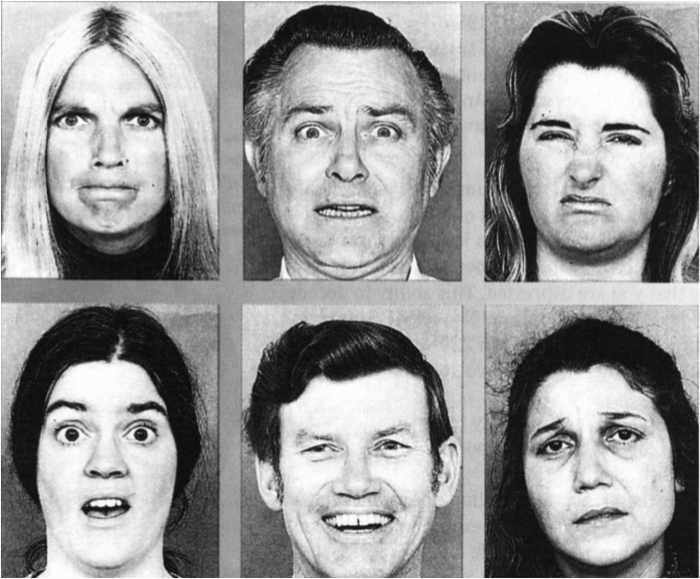
\includegraphics{emocoes.png} 
    \caption{Seis emoções básicas de Ekman.}
    \legend {Fonte: https://images.app.goo.gl/kEWB1fYVx3yawaC6A} 
\end{figure}


O modelo apresentado por \apudonline{Lazarus}{WilliamReis2017} para extrair padrões de emoções é baseado na teoria \textbf{Appraisal}, muito aceita na literatura científica, que considera as emoções como resultado de avaliações subjetivas de um determinado evento ou situação que está acontecendo em um determinado momento. Por exemplo, as pessoas podem ter interpretações diferentes do mesmo fato e isto é determinante na inferência do estado emocional ou das emoções propriamente ditas.

Segundo \citeonline{dalgleish2000handbook}, emoção é um estado breve de resposta direcionado a um objeto, ser ou evento; portanto, ela é intencional. Já o estado de humor possui uma intensidade baixa, longa duração e não é direcionado a um objeto ou não tem um elo propulsor específico capaz de o desencadear. 

Inicialmente o campo de estudos da Computação Afetiva focava mais nas emoções, porém ``atualmente ela investiga vários estados (ou fenômenos) afetivos, tais como estado de ânimo (ou humor), traços de personalidade, atitudes, entre outros fenômenos cognitivo-emocionais, por exemplo a confusão''. \cite{Jaques2019}. 

Segundo \citeonline{nunes2010computaccao}, na visão da psicologia clássica, Identidade é definida pela visão ou imagem que se tem de si mesmo e que cada pessoa possui, enquanto que na Psicologia Social e Sociologia, Identidade seria a forma como cada pessoa é vista sob os olhos da sociedade. Desta forma, existe um ``eu'' interno e um ``eu'' externo. A Identidade está intimamente relacionada à personalidade, a qual também pode ser resultante de fatores genéticos e é mais estável que as emoções ou o humor.

\apud{Hall1998}{nunes2012computaccao} separam as diversas teorias existentes acerca da personalidade em quatro grandes grupos de abordagens: (1) ênfase na psicodinâmica; (2) ênfase na realidade percebida; (3) ênfase na aprendizagem; e (4) ênfase na estrutura. Baseados nestas abordagens, os trabalhos que se apoiam na personalidade como técnica de identificação e classificação do usuário em Computação Afetiva encontram parâmetros de avaliação.

Um dos parâmetros usados para a aferição da personalidade do usuário, comum na literatura científica, é o modelo Big Five (John and Srivastava 1999) citado no trabalho de \citeonline{nunes2010computaccao} que é baseado em apenas cinco traços contidos na personalidade das pessoas e agrupados por semelhanças do indivíduo em relação aos demais.

 ``Os Cinco Grandes Fatores podem ser definidos como Extroversão, Amabilidade (ou Socialização), Conscientização (ou Realização), Neuroticismo (ou Instabilidade Emocional) e Abertura (ou Abertura à mudança)''. \apud{Hutz1998,Berger2003}{nunes2012computaccao} 
 
 ``O principal objetivo de se promover esse interfaceamento afetivo é contribuir para o aumento da coerência, consistência, predicabilidade e credibilidade das reações e respostas computacionais providas durante a interação humana via interface humano-computador''. \cite{nunes2010computaccao}

\section{Computação Afetiva no Brasil}

No Brasil, as pesquisas relacionadas à Computação Afetiva ganharam corpo nos anos 2000 e, em sua grande maioria, estão vinculadas à área da Educação conforme dispõe \citeonline{morais2017}. Este mesmo autor também avalia tais trabalhos como voltados para o quadro internacional e um dos motivos seria porque  recursos de hardware para detecção de emoções são caros no país.

``A área da Informática na Educação vem ampliando o escopo de uso de tecnologias digitais no processo de ensino e aprendizagem''. \cite{Rodrigues2017}.

Destaca-se no Brasil uma linha de pesquisa computacional que versa sobre ``estados afetivos de ânimo (animação, satisfação e desanimado), presença social, frustração, interesse, motivação, autoeficácia e fenômeno criativo''.\cite{Bercht2017}

Nesse escopo, \citeonline{Reis2018} ponderam sobre os efeitos dos estados afetivos sobre a aprendizagem individual e como a tecnologia pode interferir na regulação das emoções de modo a acelerar o processo.

\citeonline{morais2017} chama a atenção que ao fazer uma revisão sistemática das pesquisas publicadas no Brasil com o tema de Computação Afetiva aplicada à Educação nos últimos quinze anos antes de \citeyear{morais2017}, o estado do Rio Grande do Sul foi o responsável por um terço das publicações por grupo de pesquisa avaliado.

No Brasil, de acordo com um levantamento bibliográfico feito pelos autores, alguns pesquisadores possuem trabalhos notáveis. Citaremos aqui:

\begin{itemize}
  \item Patrícia A. Jaques \footnote[1]{htpp://lattes.cnpq.br/5723385125570881}, Doutora em Ciência da Computação pela Universidade Federal do Rio Grande do Sul (UFRGS) e professora na Universidade do Vale do Rio dos Sinos (Unisinos);
  \item Maria Augusta Silveira Netto Nunes
  \footnote[2]{hptt://lattes.cnpq.br/9923270028346687},
  Pós-doutora em Propriedade Intelectual pelo Instituto de Propriedade Intelectual (INPI) e professora na Universidade Federal de Sergipe (UFS);
  \item Magda Bercht
  \footnote[3]{hptt://lattes.cnpq.br/3071039194694398}
  Doutorado em Ciência da Computação pela Universidade Federal do Rio Grande do Sul (UFRGS) e professora na mesma instituição.
  \item Rachel Carlos Duque Reis
  \footnote[4]{hptt://lattes.cnpq.br/5006074852436835}
  Doutorado em Ciência da Computação pelo Instituto de Ciências Matemáticas e de Computação da Universidade de São Paulo (USP) e professora na Universidade Federal de Viçosa (UFV).
\end{itemize}

\section{Computação Afetiva e Ética}

Conversar na internet, ter suas imagens numa transmissão em tempo real ou simplesmente escrever um e-mail, tudo isto são exemplos de como precisamos pensar em ética, porque ela está para a Computação Afetiva, ainda mais do que para a tecnologia da informação. Ora, pela internet ocorrem muitos crimes e constante invasão de privacidade, pela \textbf{webcam} pode-se traçar um perfil das suas emoções, até das suas possíveis opiniões e, ao escrever o e-mail, padrões sequenciais de minerações de dados podem traçar um viés de consumo. Qual o impacto da tecnologia em nossas vidas?

``'O que é bom, Fedro, e o que não é bom – Será que é preciso pedir a alguém que nos ensine essas coisas?'. Essa reflexão é colocada por Pirsig na epígrafe de sua investigação sobre a moral (1999), e podemos tomá-la como ponto de partida''.\cite{Holanda2018}.

\citeonline{piteira2019etica} se refere à ideia da existência de máquinas “pensantes” que tomam decisões pelos humanos para trazer à tona uma série de questões éticas que devem estar presentes no centro do desenvolvimento e da aplicação da inteligência artificial nos mais diversos setores da sociedade''.

\citeonline{bembem2014tempo} cita o pensamento crítico como aquele que pode ser uma alternativa que encaminha contra as prerrogativas deterministas advindas da compreensão das tecnologias atuais e futuras. Para estes autores, na tríade conteúdo, contexto e usuário não basta criar produtos e implantá-los, mas, sim enxergar e pensar a complexidade do contexto e a gênese do produto.

``Há também na Filosofia da Informação a possibilidade de se discutir os efeitos da informação, como se dá sua passagem para o receptor, o que ela surte naqueles que a apropriam, e também quais são os efeitos dessa informação no plano da ética.''\cite{bembem2014tempo}.

``Um profissional deverá ser orientado e guiado por um conjunto de princípios que definam as suas responsabilidade profissionais''. \cite{piteira2019etica}. Tais autores citam a existência de um código de ética definido pela \textit{ACM} (\textit{Association for Computing Machinery}), \textit{The ACM Code}\footnote{https://www.acm.org/code-of-ethics} e outro definido pelo IEEE \footnote{https://www.ieee.org/about/corporate/governance/p7-8.html. [Acesso: 10-Nov-2019].}, que são as duas organizações internacionais mais conceituadas e apresentam regras básicas de conduta.

\citeonline{Holanda2018} recomendam ponderar os impactos das tecnologias, à medida que elas forem inseridas em nosso cotidiano, como positivos ou negativos e, a partir disso, traçar estratégias para nos adequarmos com bom senso. Outra ideia bastante construtiva e elucidativa é incorporar a ética no design como peça fundamental do processo de desenvolvimento, tendo em mente evitar aspirações homogeneizantes entre tecnologia e usuário; ou seja, não ter um perfil discriminador ou excludente em relação às diferenças e dificuldades.

Para \citeonline{baracho2016questoes} o	maior	desafio	na	atualidade é compreender a	informação	e	saber	como	utilizá-la.	Pois, temos acesso a muitas informações e são desenvolvidas cada vez mais tecnologias	que	envolvem compreender, questionar e buscar também	a	resolução	dos	problemas	sociais	através do	domínio	das ferramentas das	inovações disponíveis baseadas no saber.	
 
\chapter{Trabalhos Relacionados}\label{sec:TrabRel}

\section{Computação Afetiva aplicada à Educação: uma revisão sistemática das pesquisas publicadas no Brasil} \footnote{Felipe de Morais, Juarez da Silva, Helena Reis, Seiji Isotani, Patricia Jaques, 2017}

\citeonline{morais2017} O artigo faz um levantamento dos trabalhos brasileiros em Computação Afetiva aplicada à Educação nos últimos 15 anos. Para isso, foi realizado um mapeamento sistemático nos principais veículos brasileiros de divulgação científica na área, sendo eles o SBIE, WIE e a RBIE, veículos mantidos pela Comissão Especial de Informática na Educação da SBC. Foram selecionados finalmente 24 artigos, dentre eles houve os que seguiram uma base empírica, outros o modelo OCC para abordar as emoções, o modelo do Big Five para traços de personalidade, também a categoria humor, dentre outros métodos utilizados pelos artigos avaliados. Os métodos de detecção foram variados, desde \textbf{webcams} a análise de textos em e-mails e questionários para dedução de personalidade. O artigo buscou retratar o estado da arte e propor um cenário para o país em relação à pesquisa citando os principais pesquisadores, a maioria presente geograficamente na região sul. Chegou-se à conclusão de que a maioria dos trabalhos se detém nas emoções básicas e capturam os estados afetivos através do comportamento observável porque é um método menos intrusivo e os equipamentos para tal atividade são caros e fabricados no exterior. Os Sistemas Tutores Inteligentes representam a maior parte dos ambientes que levam os estados afetivos em consideração. Muitos dos artigos envolvendo detecção apresentam apenas uma proposta de trabalho, sem uma avaliação empírica.

\section{Computação Afetiva e sua influência na personalização de Ambientes Educacionais: gerando equipes compatíveis para uso em AVAs na EaD}\footnote{NUNES, M. A. S. N. et al., 2010}

\citeonline{nunes2010computaccao} trabalha muitos conceitos importantes sobre Computação Afetiva, destacando-se na área do estudo de traços da personalidade. Tanto este, como outros trabalhos da autora seguem esta linha, porém, se debruçam em desdobramentos diferentes, ou seja, as pesquisas são destinadas a fins distintos. Este artigo versa sobre o chamado EAD (Ensino a Distância) e os AVA (Ambientes virtuais de Aprendizagem) e utilizou em sua metodologia o software Personality Measure e o software Group Recommender.


\section{A Ética na Inteligência Artificial: Desafios} \footnote{PITEIRA, Martinha; APARICIO, Manuela; COSTA, Carlos J, 2019}

\citeonline{piteira2019etica} procuram discutir com atualidade os temas a respeito da ética na Inteligência Artificial, investigando as melhores abordagens da interação humano-computador e tomando como parâmetros códigos de conduta profissional e métodos científicos, os quais alguns foram citados neste trabalho.

\chapter{Resultados Esperados}\label{sec:resultEsperados}

\chapter{Cronograma}\label{sec:cronograma}
O abn\TeX\ introduziu o comando \texttt{IBGEtab} para formatação de tabelas. Um exemplo de tabela convencional do \LaTeX\ pode ser observado na \autoref{tab:cronograma} enquanto um exemplo usando o \texttt{IBGEtab} é mostrado na Tabela \ref{tab:cronogramaIBGE}.

\begin{table}[htbp]
  \centering
    \caption[Cronograma Normal]{Cronograma do Projeto em Meses}
    \label{tab:cronograma}
    \begin{tabular}{lcccccccccccc} %|c|c|c|c|c|c|c|c|c|c|c|c
    \toprule
    \textbf{Atividade} & \textbf{1} & \textbf{2} & \textbf{3} & \textbf{4} & \textbf{5} & \textbf{6} & \textbf{7} & \textbf{8} & \textbf{9} & \textbf{10} & \textbf{11} & \textbf{12} \\
    \midrule
        Revisão Bibliográfica & $\bullet$ & $\bullet$ & & & & & & & & & & \\
        Métodos & & & $\bullet$ & $\bullet$ & & & & & & & & \\
        Testes & & & & $\bullet$ & $\bullet$ & $\bullet$ & & & & & & \\
        Resultados & & & & & & & $\bullet$ & $\bullet$ & & & & \\
        Conclusão & & & & & & & $\bullet$ & $\bullet$ & $\bullet$ & & & \\
        Banca & & & & & & &&&& $\bullet$ & $\bullet$ & $\bullet$ \\
    \bottomrule
    \end{tabular}%
    \fonte{Próprio Autor}
\end{table}%

\begin{table}[htbp]
    \IBGEtab{
    \caption[Cronograma (IBGE)]{Cronograma do Projeto em Meses usando o comando IBGEtab para a formatação da tabela}
    \label{tab:cronogramaIBGE}
    }{
    \begin{tabular}{lcccccccccccc} %|c|c|c|c|c|c|c|c|c|c|c|c
    \toprule
    \textbf{Atividade} & \textbf{1} & \textbf{2} & \textbf{3} & \textbf{4} & \textbf{5} & \textbf{6} & \textbf{7} & \textbf{8} & \textbf{9} & \textbf{10} & \textbf{11} & \textbf{12} \\
    \midrule
        Revisão Bibliográfica & $\bullet$ & $\bullet$ & & & & & & & & & & \\
        Métodos & & & $\bullet$ & $\bullet$ & & & & & & & & \\
        Testes & & & & $\bullet$ & $\bullet$ & $\bullet$ & & & & & & \\
        Resultados & & & & & & & $\bullet$ & $\bullet$ & & & & \\
        Conclusão & & & & & & & $\bullet$ & $\bullet$ & $\bullet$ & & & \\
        Banca & & & & & & &&&& $\bullet$ & $\bullet$ & $\bullet$ \\
    \bottomrule
    \end{tabular}%
    }{
    \fonte{Próprio Autor}}
\end{table}%

% ----------------------------------------------------------
% ELEMENTOS PÓS-TEXTUAIS
% ----------------------------------------------------------
\postextual

% Referências bibliográficas

%\bibliography{referencias}
%\linespread{1}
%\printbibliography
\bibliography{referencias}
% Caso sejam necessários apêndices ou anexos em seu documento
% Use os ambientes abaixo

%% Apêndices
%
%% Inicia os apêndices
%\begin{apendicesenv}
%
%% Imprime uma página indicando o início dos apêndices
%\partapendices
%
%\chapter{Primeiro Apêndice}
%
%\chapter{Segundo Apêndice}
%
%\end{apendicesenv}
%
%% ----------------------------------------------------------
%% Anexos
%% ----------------------------------------------------------
%\begin{anexosenv}
%
%% Imprime uma página indicando o início dos anexos
%\partanexos
%
%\chapter{Primeiro Anexo}
%\lipsum[30]
%
%\chapter{Segundo Anexo}
%\lipsum[31]
%
%\end{anexosenv}

\end{document}
